% !TeX root = repressed-anger.tex

\section{Sentiment Analysis}
\label{sec:sentiment_analysis}

\acrfull{sa}, sometimes referred as \acrfull{om}, is the field of study that aims determine the attitude of the author respect to some topic. During the last decade, due mainly to the rapid increase of the social media, the research of this area, which includes linguistics and \acrfull{nlp}, has gain more relevance as it has a wide range of applications that can be used commercially.

Almost the human actions are influenced by opinions. A practical example of this behavior that get repeated in daily basics occurs when before making a decision we want to know other' to contrast our thoughts. In business, when an organization requires to public or consumer opinion, it conducted different types of surveys to gather this information. However, nowadays we do not precise to ask personally to people around us to discuss about a product. Thanks to micro-blogs, Twitter and reviews in social networks, we can broaden the amount of external opinions for decision making. Due to the amusing amount of information available, sometimes we could face some challenges, such as finding reliable sources summarizing and filtering the relevant information. The same way we consume this information, companies also search for new ways to obtain and process such information efficiently without human intervention, to achieve this automated analysis is needed\cite{liu2012sentiment}.

\subsection{Tasks}
\label{subsec:sentiment_analysis_tasks}

\begin{figure}[!htp]
  \center
  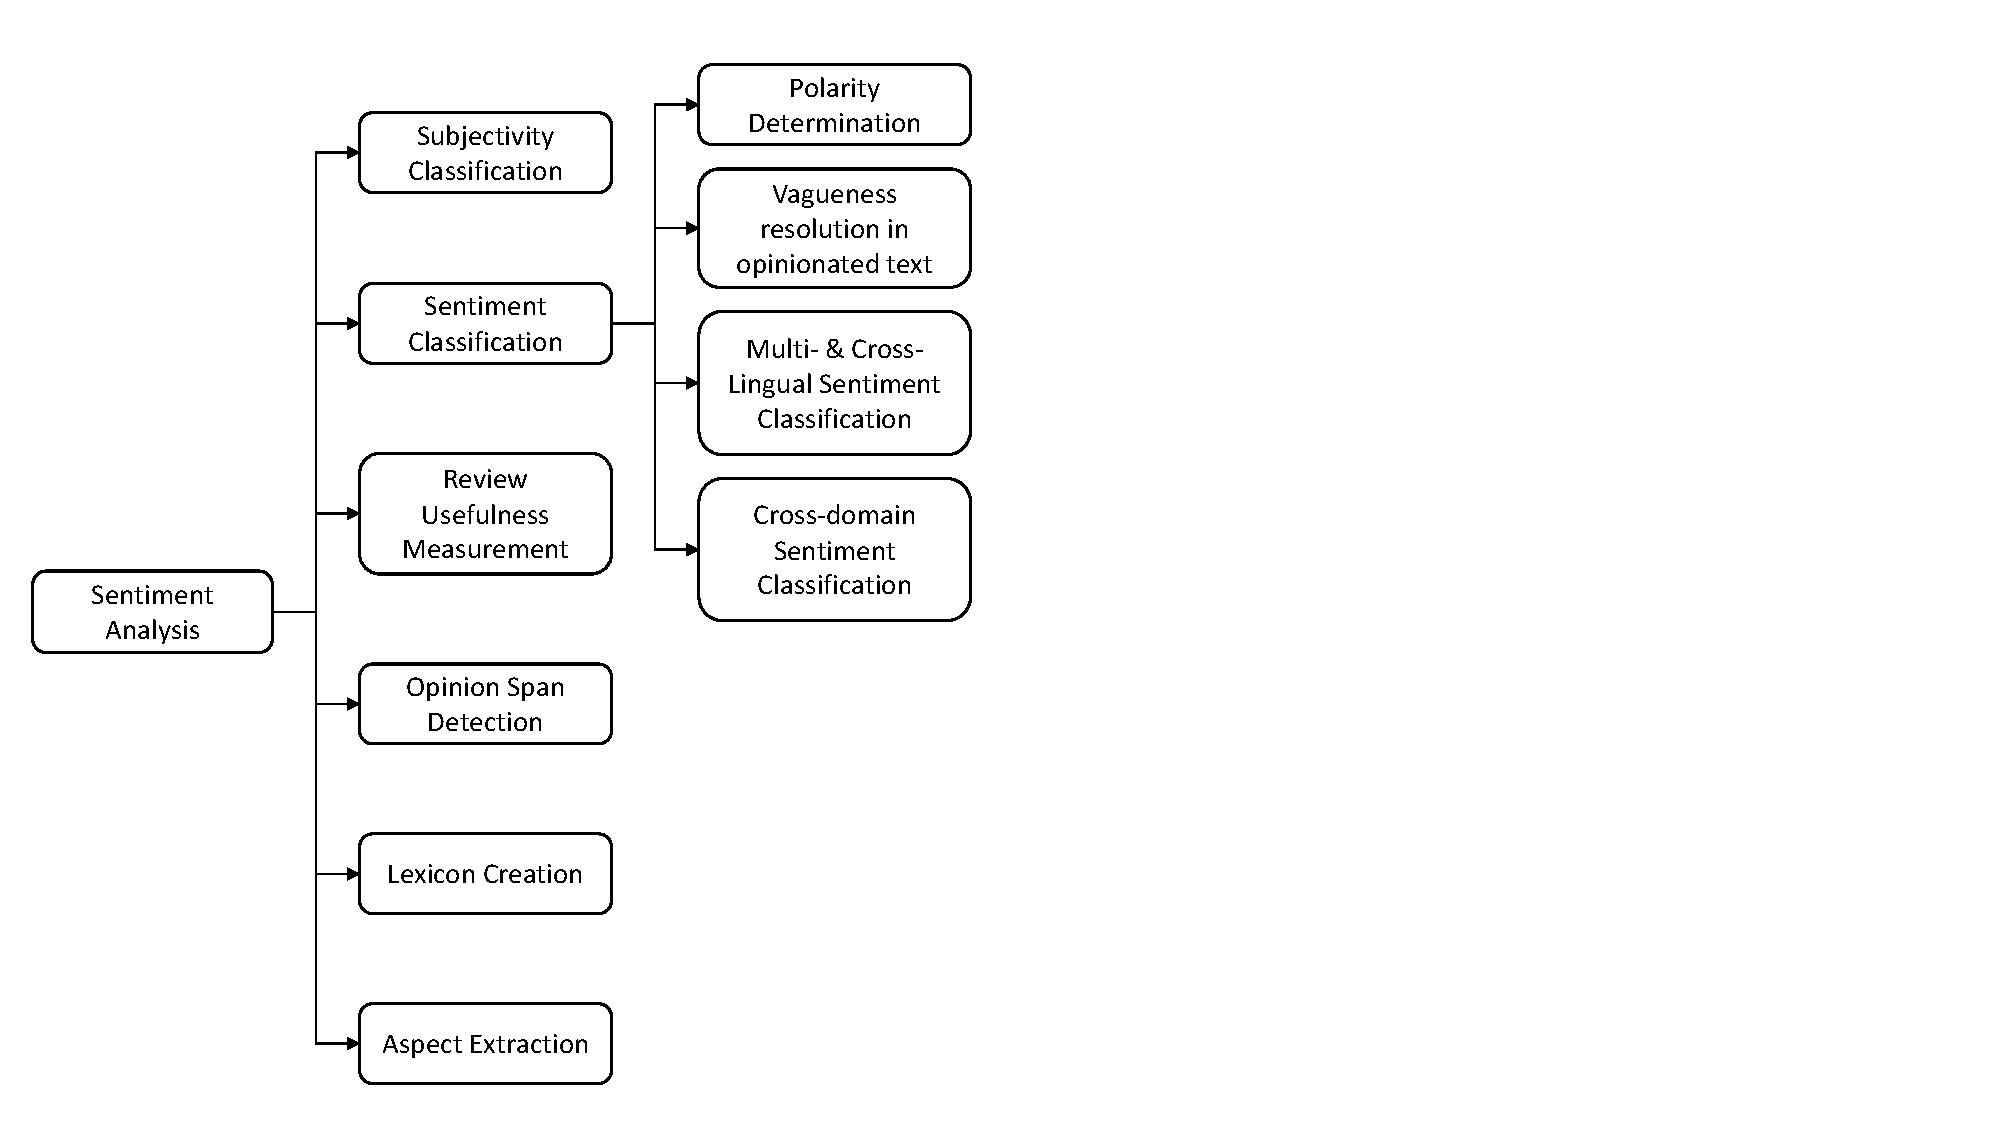
\includegraphics[width=1\textwidth]{figures/sentiment_analysis_tasks}
  \caption{Sentiment analysis tasks.}
  \label{fig:sentiment_analysis_tasks}
\end{figure}

Depending on the problem definition, different tasks have been defined related to sentiment analysis. According to \cite{ravi2015survey}, after the revision of more than three hundred papers related to this topic, the survey carried out concludes that the main tasks can be categorized as (a) subjectivity classification, (b) sentiment classification, (c) review usefulness measurement, (d) opinion spam detection, (e) lexicon creation and (f) aspect extraction, as shown in the figure \ref{fig:sentiment_analysis_tasks}. 

\subsubsection{Subjectivity classification}
\label{subsubsection:subject_classification}

According to \cite{montoyo2012subjectivity}, subjectivity classification aims to determine the "private state" of the author of a text. The Subjectivity analysis is the process of distinguish objective language from the opinion oriented. Even though there is much less literature about this field compared to other \acrshort{sa} task, it has proven to be more difficult than determine the measuring the polarity of a document and, thus, improvements achieved in this field will positively impact on sentiment classification.

\subsubsection{Sentiment classification}
\label{subsubsection:sentiment_classification}

Sentiment classification consist in determine the orientation of a sentiment of a given text into two or more classes. This classification has been performed in multiple classes, such as, binary (positive or negative), ternary (positive, neutral and negative), n-ary \cite{nakov2016semeval}, among others.

\subsubsection{Review usefulness measurement}
\label{subsubsection:review_usefulness_measurement}

Review usefulness measurement tends sometimes be confused with opinion spam detection, however there are some slight differences. Of course false review are always rated as useless, as their objective is just to boast or ridicule a product. Although, there are also bad reviews that might not necessary be spam, as they reflect the honest opinion of the author. Thus, this subtask complement the opinion spam detection.

\subsubsection{Opinion spam detection}
\label{subsubsection:opinion_spam_detection}

In order to boost sales, some companies have invested on unmoral marketing techniques that consist in publishing false reviews about their own products or from the competence. In order to detect fake reviews, researches have focus their effort on (a) analyzing the content of the review, finding hidden lies by using \acrshort{nlp}, (b) meta-data of the review, such as start rating, author information, date of writing, among many others \cite{hu2011fraud}, however this information sometimes is not accessible, and (c) comparison with real-life information about the product. 

\subsubsection{Lexicon creation}
\label{subsubsection:lexicon_creation}

A lexicon is a collection of words that determines the polarity of each one of them. Lexicons are used as an approach to detect the sentiment polarity of a given document \cite{kaji2007building}.

\subsubsection{Aspect extraction}
\label{subsubsection:aspect_extraction}

Aspect extraction is a key to detect author's opinion regarding various characteristics of a product based on the collection of opinion words and entities and identification and extraction of the aspects of those entities \cite{mukherjee2012aspect}.

\subsection{Techniques}
\label{subsec:sentiment_analysis_techniques}

\begin{figure}[!htp]
  \center
  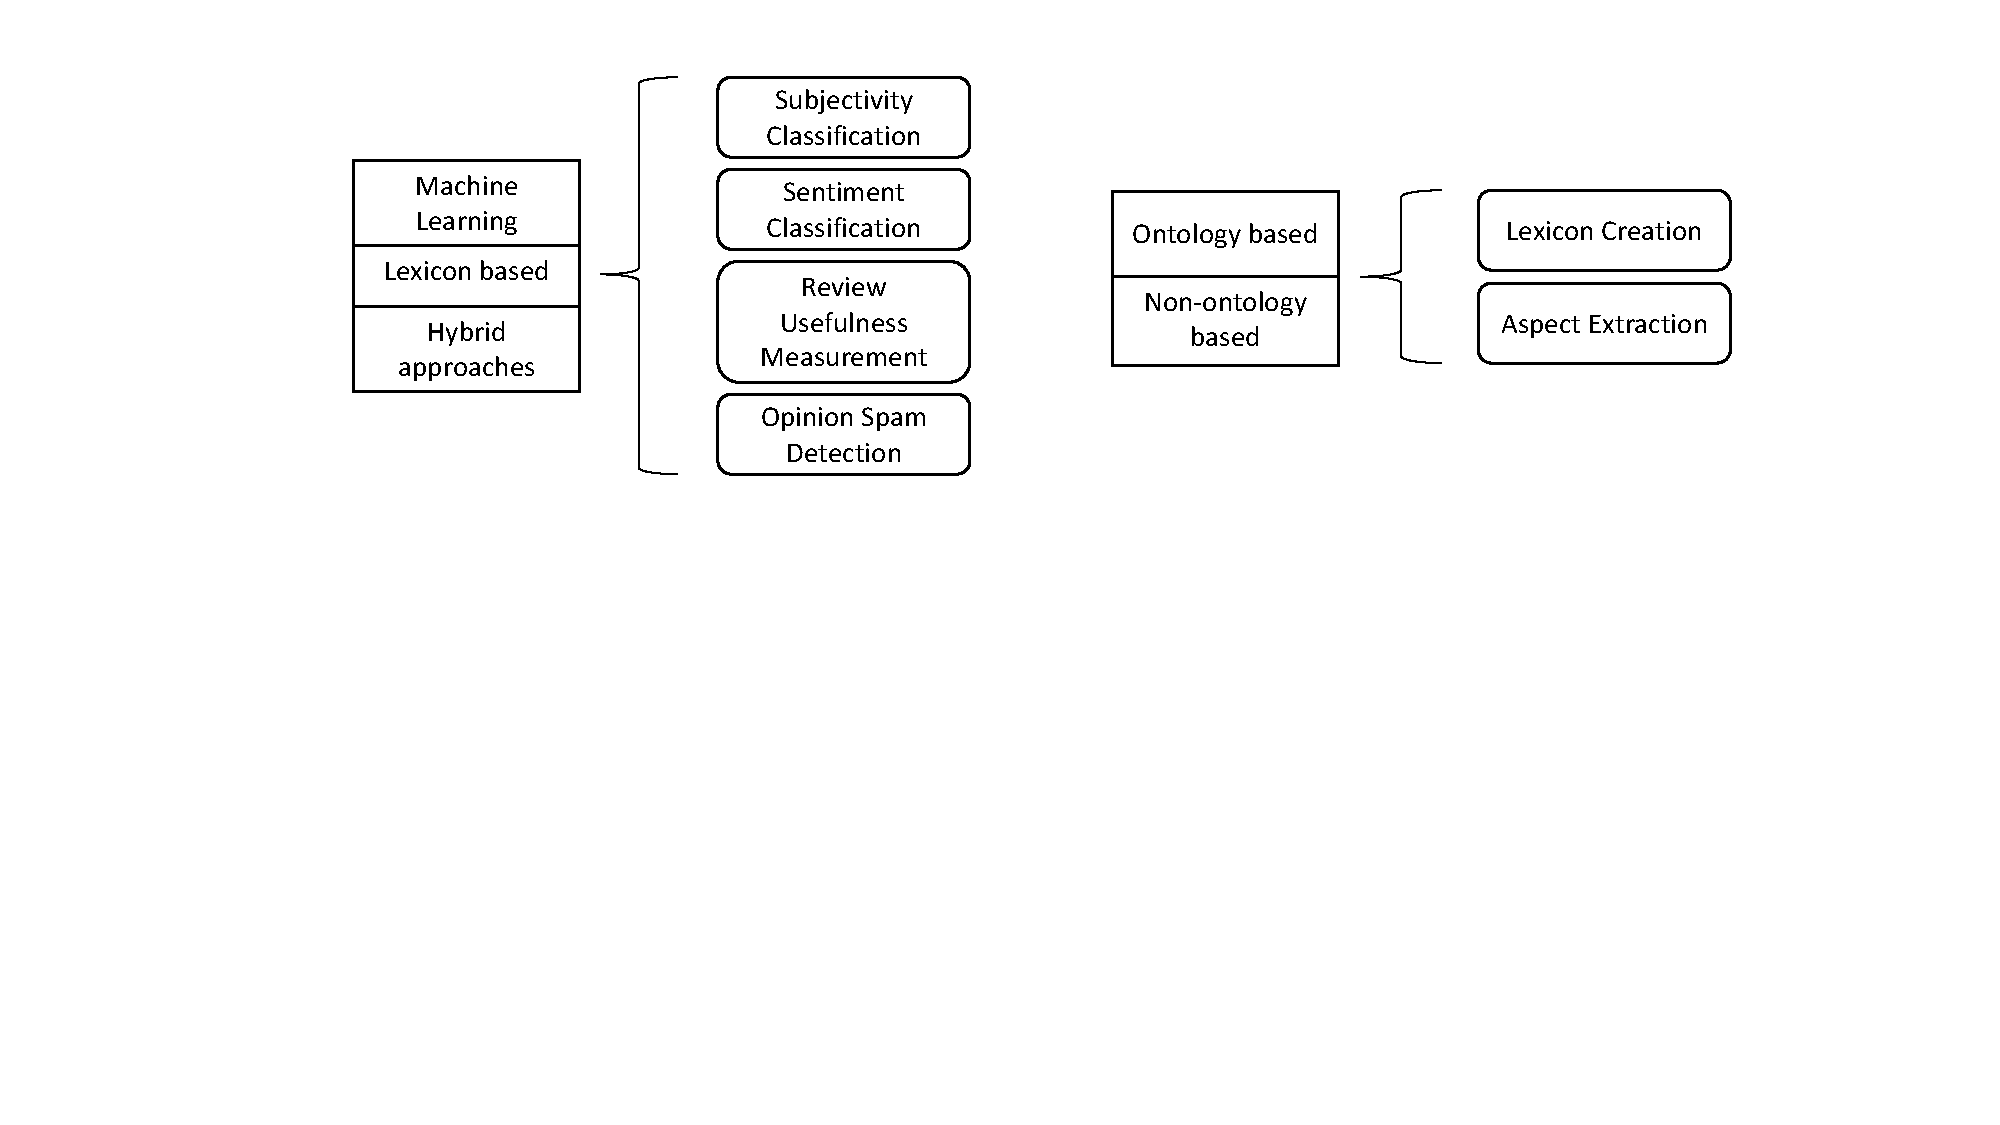
\includegraphics[width=0.9\textwidth]{figures/sentiment_analysis_approaches}
  \caption{Sentiment analysis approaches for each task.}
  \label{fig:sentiment_analysis_approaches}
\end{figure}

To solve all these problems in the most efficient way, multiple approaches have been conducted, such as \cite{tripathy2016classification}; \cite{mullen2004sentiment} or \cite{pouransari2014deep}. The figure \ref{fig:sentiment_analysis_approaches} illustrates which techniques have been used for each previously named tasks.

\FloatBarrier

The figure \ref{fig:sentiment_analysis_techniques} collects the most common techniques used for \acrshort{sa} based the survey conducted by Walaa Medhat et al. (2014). For the purpose of this project, we will focus on making an introduction to those approaches related to sentiment classification, more precisely to \acrfull{ml}, lexicon-based and hybrid approaches.

\begin{figure}[!htp]
  \center
  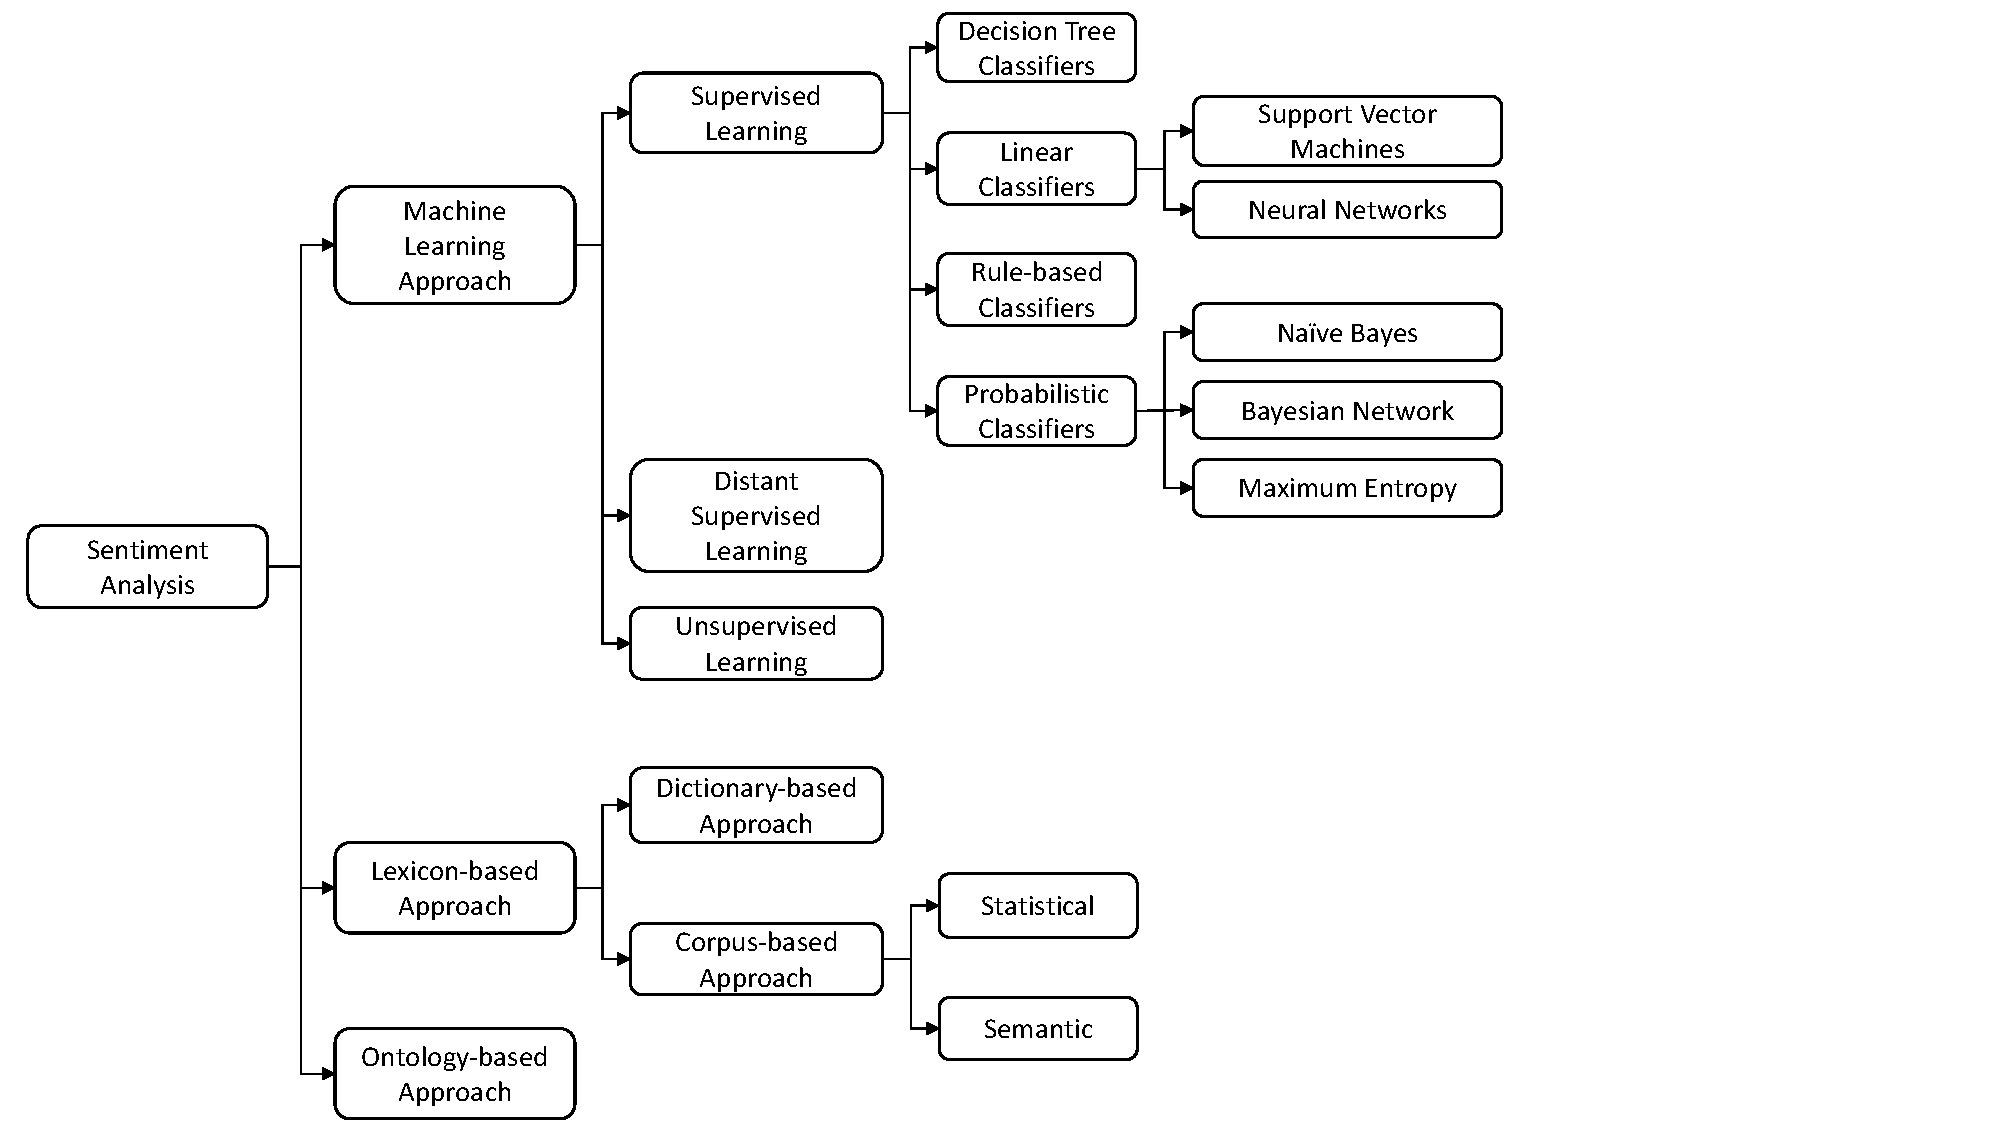
\includegraphics[width=1\textwidth]{figures/sentiment_analysis_techniques}
  \caption{Sentiment analysis techniques\cite{medhat2014sentiment}.}
  \label{fig:sentiment_analysis_techniques}
\end{figure}

\FloatBarrier

\subsubsection{Machine learning approach}
\label{subsubsec:techniques_machine_learning}

Thanks to the good performance machine learning techniques have proved to achieve, more and more researches have gain interest on this technology. The classification process (see \ref{sec:algorithms}) used, consist on extracting a series of features vectors from the dataset and a to create a model that is able to identify different patters among theses features. The selection of relevant features is key as it directly affect the performance the model can score. Some good known features for model generation are based on n-grams, such as unigrams, bi-grams and tri-grams \cite{furnkranz1998study}.

\begin{enumerate}[label=\textbf{\arabic*}.]
  \item \textbf{Data gathering:} During this phase, first publicly available datasets are searched from related literature. Then if needed, to complement this data, an analysis of the social media that contains information regarding the research topic is conducted. After analyzed the sources from which data can be extracted, a crawler adapted to deal with those networks is used to collect the data. This data, usually mostly or partially, requires to be labeled with a predefined set of classes, a task generally done by crowd-sourcing.
  \item \textbf{Pre-processing:} Most of the raw data obtained from social media contains information is not relevant or cannot be directly processed by the classifier. In this step, tasks like word spell checking, \acrfull{url} and hash-tags removal, keyword extraction, language filtering, tokenization, among many others are carried out.
  \item \textbf{Classifier training:} With the dataset most commonly split into training, validation and test, the training and validation sets will be provided as an input to the classification algorithm as the learning process, which concludes with the generation of a model.
  \item \textbf{Classification:} With the previously generated model on the learning process, the classifier can now be used to predict new data.
  \item \textbf{Result evaluation:} To measure how accurate the learning algorithm performed, the output of the system is compared with dataset labels by means of a defined evaluation function and representation format.
\end{enumerate}

\subsubsection{Lexicon based approach}
\label{subsubsec:techniques_lexicon_based}

Sentiment analysis based on lexicon approach consist on the use of a collection of words, a dictionary, that contain a pre-tagged lexicon to classify a given text. The input document is tokenized and, thus, every token is compared with the lexicon forming the dictionary. Depending on how the lexicon is defined, the result of the comparison can be either positive or negative. If positive match is given, the total score of the text classification is increased, if negative match occurs, then the score decreases. Although this technique could be considered simplistic, some simplistic tests \cite{hatzivassiloglou2000effects} have proven to be successful in achieving high precision. 

\subsubsection{Hybrid approach}
\label{subsubsec:techniques_hybrid}

As \cite{thakkar2015approaches} suggest, both, machine learning and lexicon based approaches have their advantages and disadvantages. Thus, researchers have tried merging different methods to order to find more precise and efficient ways of classify sentiments. The combination of techniques are variated that include architectures that mix lexicons to automatically label data that is used as a learning input into a Naive Bayes classifier as shown in \cite{pak2010twitter}; the author of \cite{khan2014tom} uses the combination of three classifiers, enhanced emoticon classifier, improved polarity classifier and a SentiWordNet classifier to determinate the polarity of a given tweet or \cite{prabowo2009sentiment}, which used multiple rule based classifiers approaches combined with \acrshort{svm} executed on multiple hybrid sequential executions on a semi-automatic dataset.